\documentclass{article}

% Language setting
% Replace `english' with e.g. `spanish' to change the document language
\usepackage[english]{babel}
\usepackage{multicol}
\setlength{\columnsep}{1cm}

% Set page size and margins
% Replace `letterpaper' with `a4paper' for UK/EU standard size
\usepackage[A4paper,top=2cm,bottom=2cm,left=2cm,right=2cm,marginparwidth=1.75cm]{geometry}

% Useful packages
\usepackage{caption}
\usepackage{amsmath}
\usepackage{siunitx}
\usepackage{wrapfig}
\usepackage{float}
\usepackage{graphicx}
\graphicspath{{images/}}
\usepackage{subcaption}
\usepackage[colorlinks=true, allcolors=blue]{hyperref}
\usepackage{xcolor}
\usepackage{listings}

\title{Modelling and controlling a reaction wheel on an inverted pendulum}
\author{Michel Vollmuller, 1809572}

\begin{document}
\maketitle

\begin{abstract}

In this paper an experimental setup is described in which a pendulum with a reaction wheel on top is balanced by using the torque of an reaction wheel. For the control mechanism a PID controller was used. A digital twin of the system was modelled in Python.\end{abstract}

\begin{multicols}{2}

\section{Experimental setup}

The setup consists of a 3D-printed model see figure \ref{fig:3d ontwerp}, with a pendulum on a stand that can be clamped to a table. The pendulum arm is 55 mm long, measured from the center of the pivot point to the center of the reaction wheel. An MPU6050 is attached to the arm, which can read the angle of the pendulum. At the top of the pendulum is a 3-phase 2804 100kv BLDC motor. Connected to this motor is an reaction wheel with a radius of 50 mm. To see the motor's position for better control, there is a magnet in the motor shaft, which an AS5600 sensor can read to find the angle of the motor.
To control the entire system, an Arduino Nano is used, and a motor driver is employed to send high power levels to the motor.

\begin{figure}[H]
\centering
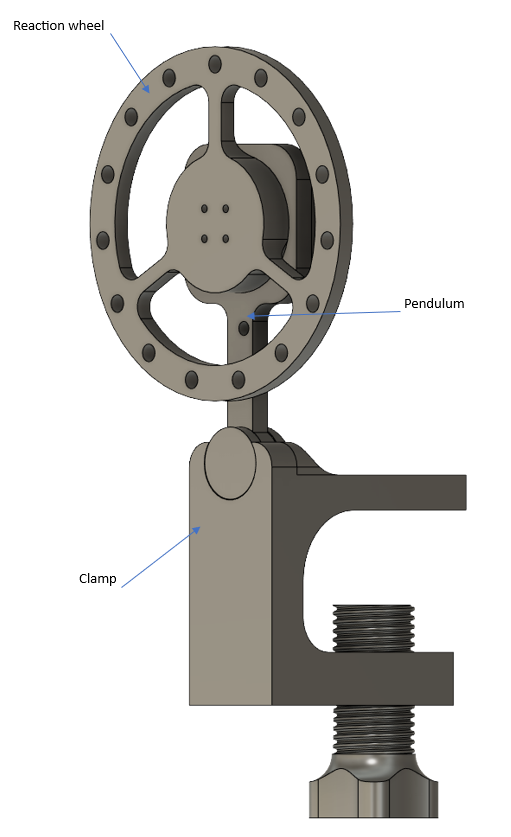
\includegraphics[scale=0.42]{Pendulum v13 schuin}
\caption{Ontwerp van het 3d model}
\label{fig:3d ontwerp}
\end{figure}

\section{Theory}

Simulating an inverted pendulum with an reaction wheel involves modeling the dynamics of both the pendulum and the reaction wheel. In this scenario, the inverted pendulum represents a system where the pendulum is balanced. The reaction wheel is used to control and stabilize the system.

\subsection{Pendulum Dynamics:}

\begin{figure}[H]
\centering
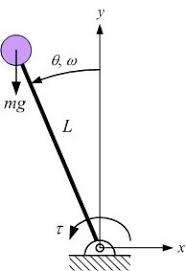
\includegraphics[scale=0.5]{images}
\caption{Pendulum Physics}
\label{fig:Pendulum Physics}
\end{figure}
The dynamics of a simple pendulum can be described using the equation:

\[
I \cdot \ddot{\theta} = -m \cdot g \cdot L \cdot \sin(\theta)
\]

Where:
\begin{align*}
&I \text{ is the moment of inertia of the pendulum,  } \, \text{kg} \cdot \text{m}^2\\
&\ddot{\theta} \text{ is the angular acceleration,  } \, \text{rad/s}^2\\
&m \text{ is the mass of the pendulum bob,  } \, \text{kg}\\
&g \text{ is the acceleration due to gravity,  } \, \text{m/s}^2\\
&L \text{ is the length of the pendulum,  } \, \text{m}\\
&\theta \text{ is the angular displacement.  } \, \text{rad}
\end{align*}
      

\subsection{Reaction Wheel Dynamics:}

The dynamics of the reaction wheel can be described using the equation:

\[
I_{\text{rw}} \cdot \dot{\omega}_{\text{rw}} = \tau_{\text{rw}}
\]

Where:
\begin{align*}
&I_{\text{rw}} \text{ is the moment of inertia of the reaction wheel,} \\
&\dot{\omega}_{\text{rw}} \text{ is the angular acceleration of the reaction wheel,} \\
&\tau_{\text{rw}} \text{ is the torque applied by the reaction wheel.}
\end{align*}

\subsection{Torque Interaction:}

The torque from the reaction wheel can be used to control the angular acceleration of the pendulum. The net torque affecting the system is the sum of the torque from the reaction wheel and any external torques acting on the pendulum. Assuming no external torques, we can write:

\[
\tau_{\text{total}} = \tau_{\text{rw}}
\]

\subsection{Combining Equations:}

\begin{figure}[H]
\centering
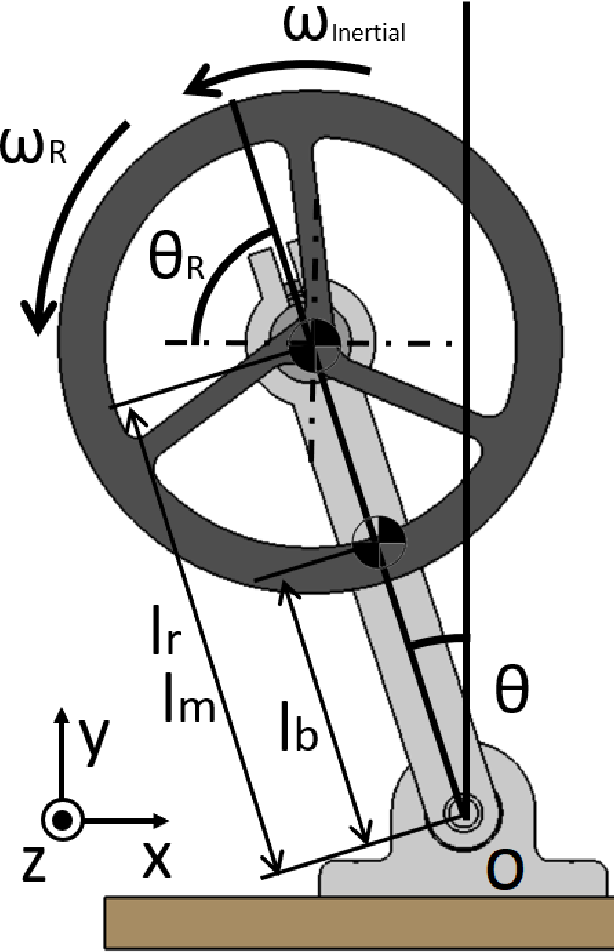
\includegraphics[scale=0.195]{inverted pendulum reactionwheel}
\caption{Pendulum + reaction wheel Physics}
\label{fig:Pendulum + reaction wheel Physics}
\end{figure}

Combine the equations for the pendulum and reaction wheel dynamics. For simplicity, you may need to make some assumptions, such as neglecting air resistance and friction.

\[
I \cdot \ddot{\theta} = -m \cdot g \cdot L \cdot \sin(\theta) + \tau_{\text{rw}}
\]

\subsection{Simulation:}

By using these equations, it's possible to simulate the model in software tools such as 20-sim, Python, or Excel, employing numerical methods like the Euler method to solve the coupled system of differential equations over time. Techniques such as LQR or PID can be utilized to control the model, making it stable and allowing simulation of how the model will respond to external forces.

See appendix B for the implementation in python.

\subsection{Control:}

In my simulation, I used PID control. 
This technique first calculates the error (setpoint - current output) of the system, and then a control output is computed based on proportional (Kp), integral (Ki), and derivative (Kd) gains. 
By tuning these values, the system can be made more or less stable.
The values I used for the PID controller were:
\begin{align*}
\text{ Kp = 1.40}\\
\text{ Ki = 0.01}\\
\text{ Kd = 3.60}
\end{align*}



The control output of the PID will be used to drive the motor, resulting in torque from the reaction wheel that, in turn, affects the acceleration of the pendulum. This allows the control over the system.


\section{Measurements simulation}
For the simulation of the system, I referred to an article by Korn, Nopparuj, Paweekorn, and Punyawat, who are students at the Institute of Field Robotics, King Mongkut’s University of Technology Thonburi (FIBO). In their work, they explain the swing-up and balancing of a reaction wheel inverted pendulum, providing a simulation that demonstrates the operation with both LQR and PID control. In my own simulation, I focus only on the balancing aspect using PID. however, it's fun and interesting to observe the differences between the FIBO simulation and mine.

\begin{figure}[H]
\centering
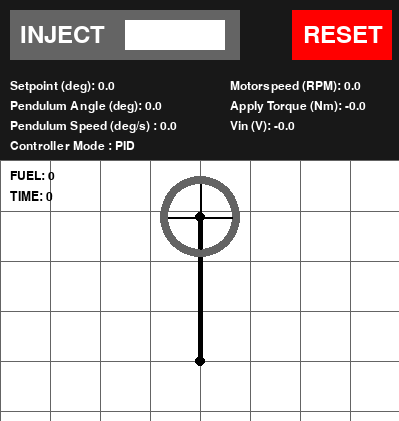
\includegraphics[scale=1.5]{simulatie foto}
\caption{Here is how the Python simulation looks.}
\label{fig:Graphic Simulation}
\end{figure}

In figure \ref{fig:Stepresponse PID controlled simulation Michel} and \ref{fig:Stepresponse PID controlled simulation FIBO}, you can see how both simulations respond to an additional, external force applied to the end of the pendulum. It isn't an fair comparison because the applied forces are not exactly the same. However, it's interesting to note that the observed behavior is nearly identical. Also, it appears that the FIBO simulation is somewhat more accurate. Nevertheless, this is still an interesting comparison, indicating that my simulation seems to be accurate.

\begin{figure}[H]
\centering
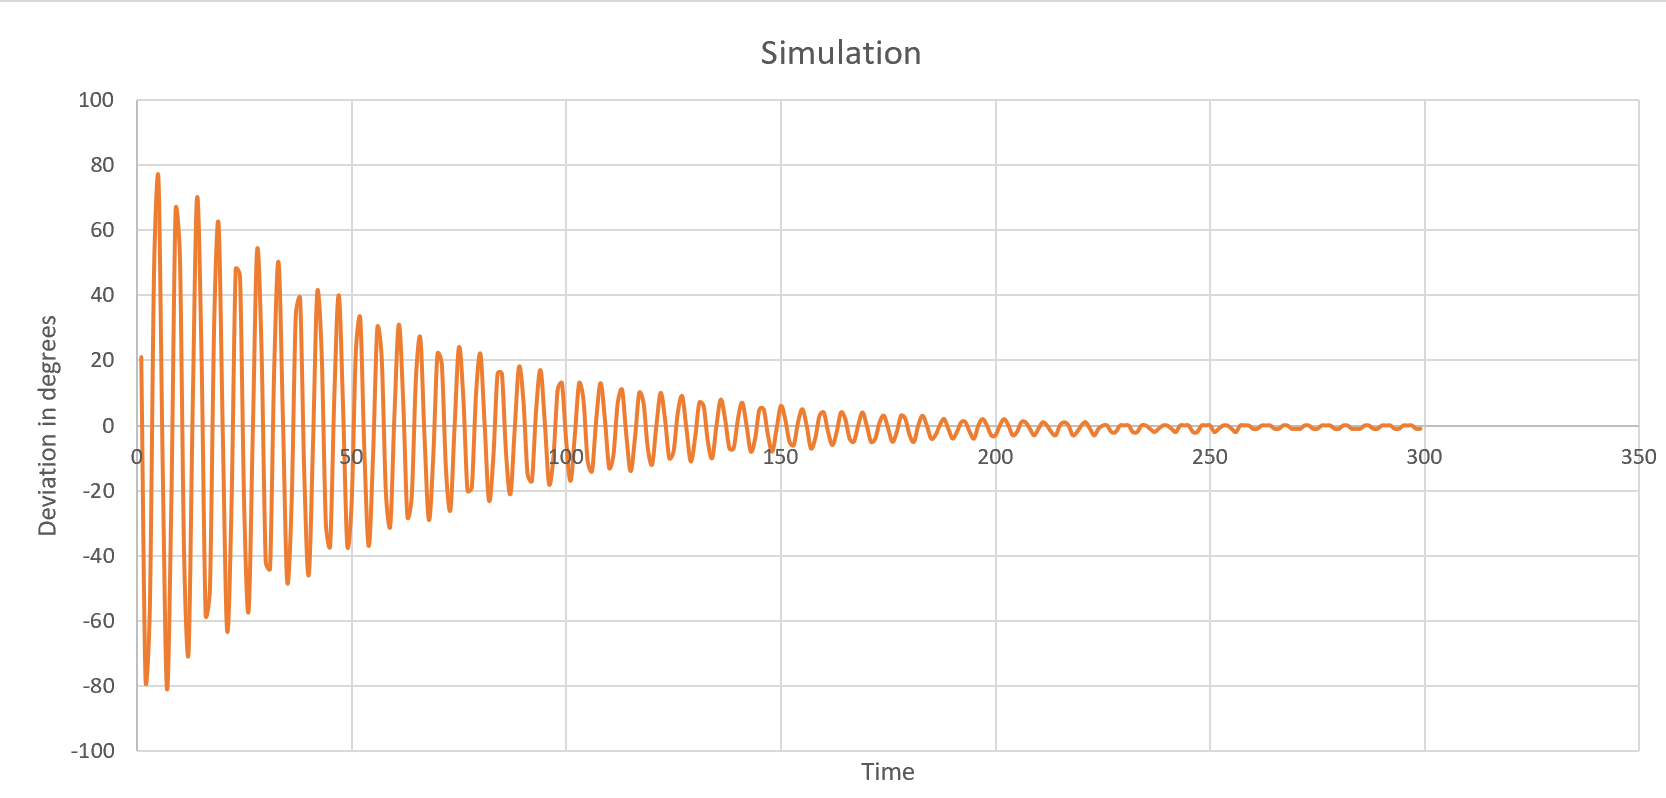
\includegraphics[scale=0.37]{Stepresponse Michel}
\caption{Stepresponse PID controlled simulation programmed by Michel.}
\label{fig:Stepresponse PID controlled simulation Michel}
\end{figure}

\begin{figure}[H]
\centering
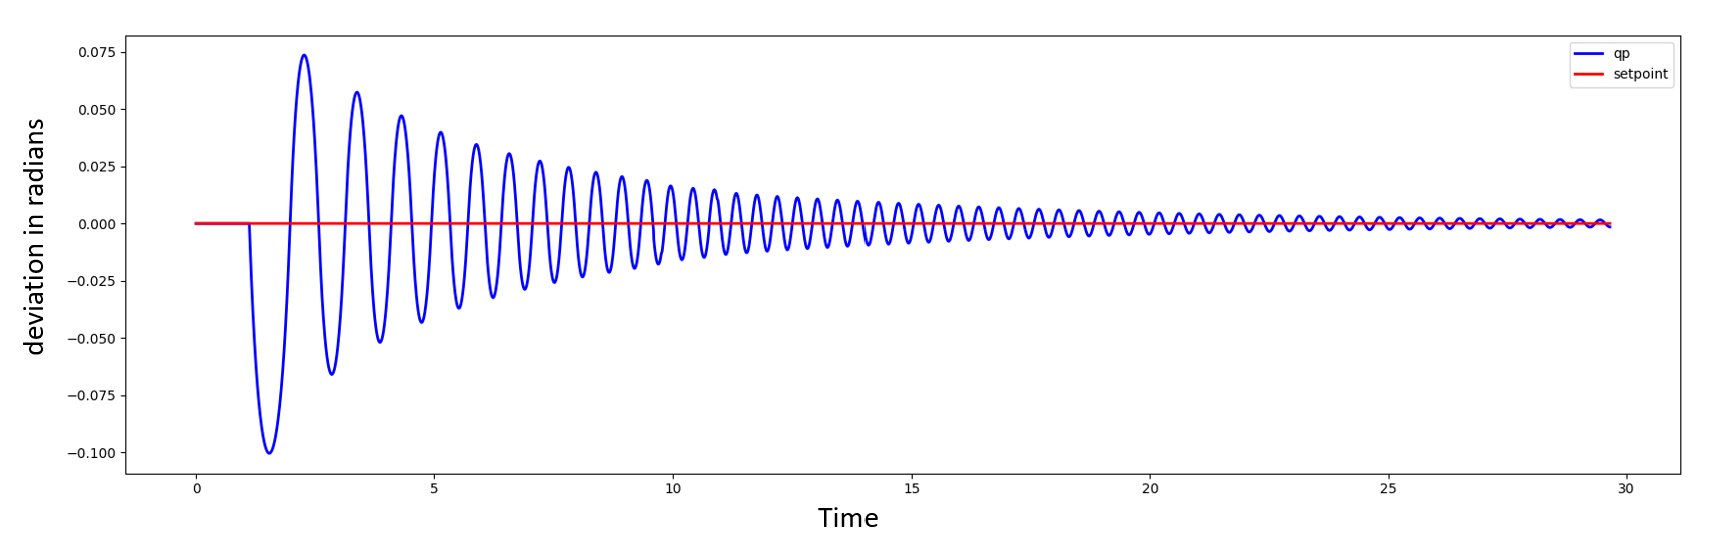
\includegraphics[scale=0.37]{Stepresponse FIBO}
\caption{Stepresponse PID controlled simulation programmed by the FIBO.}
\label{fig:Stepresponse PID controlled simulation FIBO}
\end{figure}


The interesting aspect of the FIBO article is that they have also conducted calculations for an LQR simulation. In figure \ref{fig:Stepresponse LQR controlled simulation FIBO}, you can observe the simulation where an additional external force is applied to the end of the pendulum. In figure \ref{fig:Stepresponse LQR controlled simulation FIBO}, you can observe how the model responds to an external force with LQR control compared to PID control, as depicted in figure \ref{fig:Stepresponse PID controlled simulation Michel} and \ref{fig:Stepresponse PID controlled simulation FIBO}. It is clearly visible that with LQR, the pendulum quickly returns to its setpoint without the need for significant oscillations before reaching the desired position.

\begin{figure}[H]
\centering
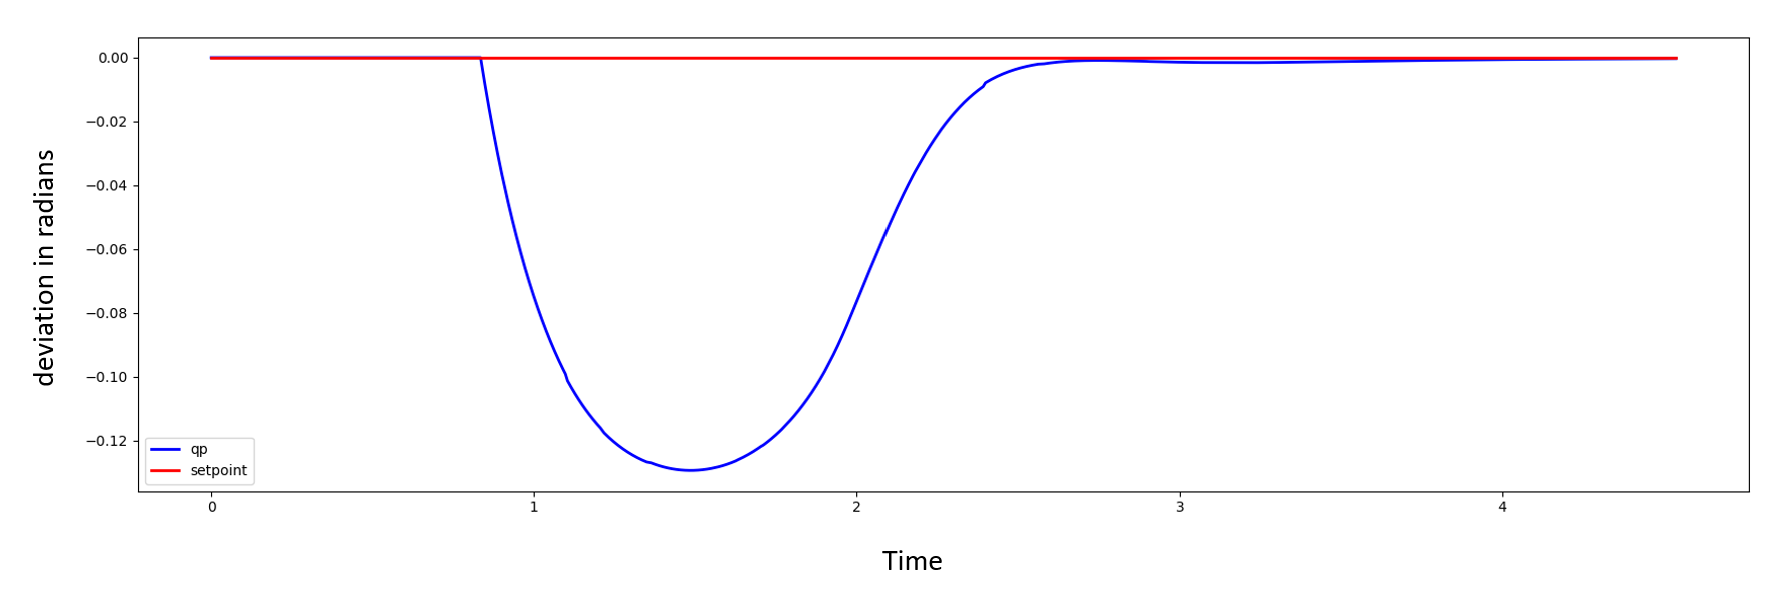
\includegraphics[scale=0.37]{Stepresponse FIBO LQR}
\caption{Stepresponse LQR controlled simulation FIBO.}
\label{fig:Stepresponse LQR controlled simulation FIBO}
\end{figure}


LQR stands for Linear Quadratic Regulator, and it is a control algorithm used in the field of control theory to design controllers for linear dynamic systems. LQR aims to minimize a quadratic cost function that represents the trade-off between control effort and system performance.

The key components of an LQR controller include:
\begin{enumerate}
    \item State-space representation: The dynamic behavior of a system is described using state-space equations. These equations represent how the state variables of the system change over time.
    \item Cost function: LQR formulates a cost function that involves the weighted sum of the state variables and control inputs. The goal is to find control inputs that minimize this cost function.
    \item Weighting matrices: LQR uses weighting matrices to assign importance to different components of the cost function. The choice of these matrices influences the balance between achieving good system performance and minimizing control effort.
    \item Optimization: The LQR algorithm involves solving a matrix Riccati differential equation to find the optimal state feedback matrix. This matrix determines how the control input is computed based on the current state of the system.
\end{enumerate}

The resulting LQR controller provides a linear feedback law that is often represented as a linear combination of the state variables. This feedback control law aims to stabilize the system and optimize its performance according to the specified cost function.

\section{Physical setup}
At the beginning of this project, the intention was to create a relatively small and compact model of a balancing pendulum using a reaction wheel, allowing for easy transportation and demonstrations in various locations. Unfortunately, this has resulted in nothing more than numerous lessons. Due to the relatively small size of the model, it requires a high level of precision, which is not achievable with the current hardware.

In figure \ref{fig:Phisical setup}, you can see the model in real life. The plan was to attach the model to a surface using a clamp. However, the 3D-printed clamp turned out not to be strong enough to stand stable. Hence the use of tape.

\begin{figure}[H]
\centering
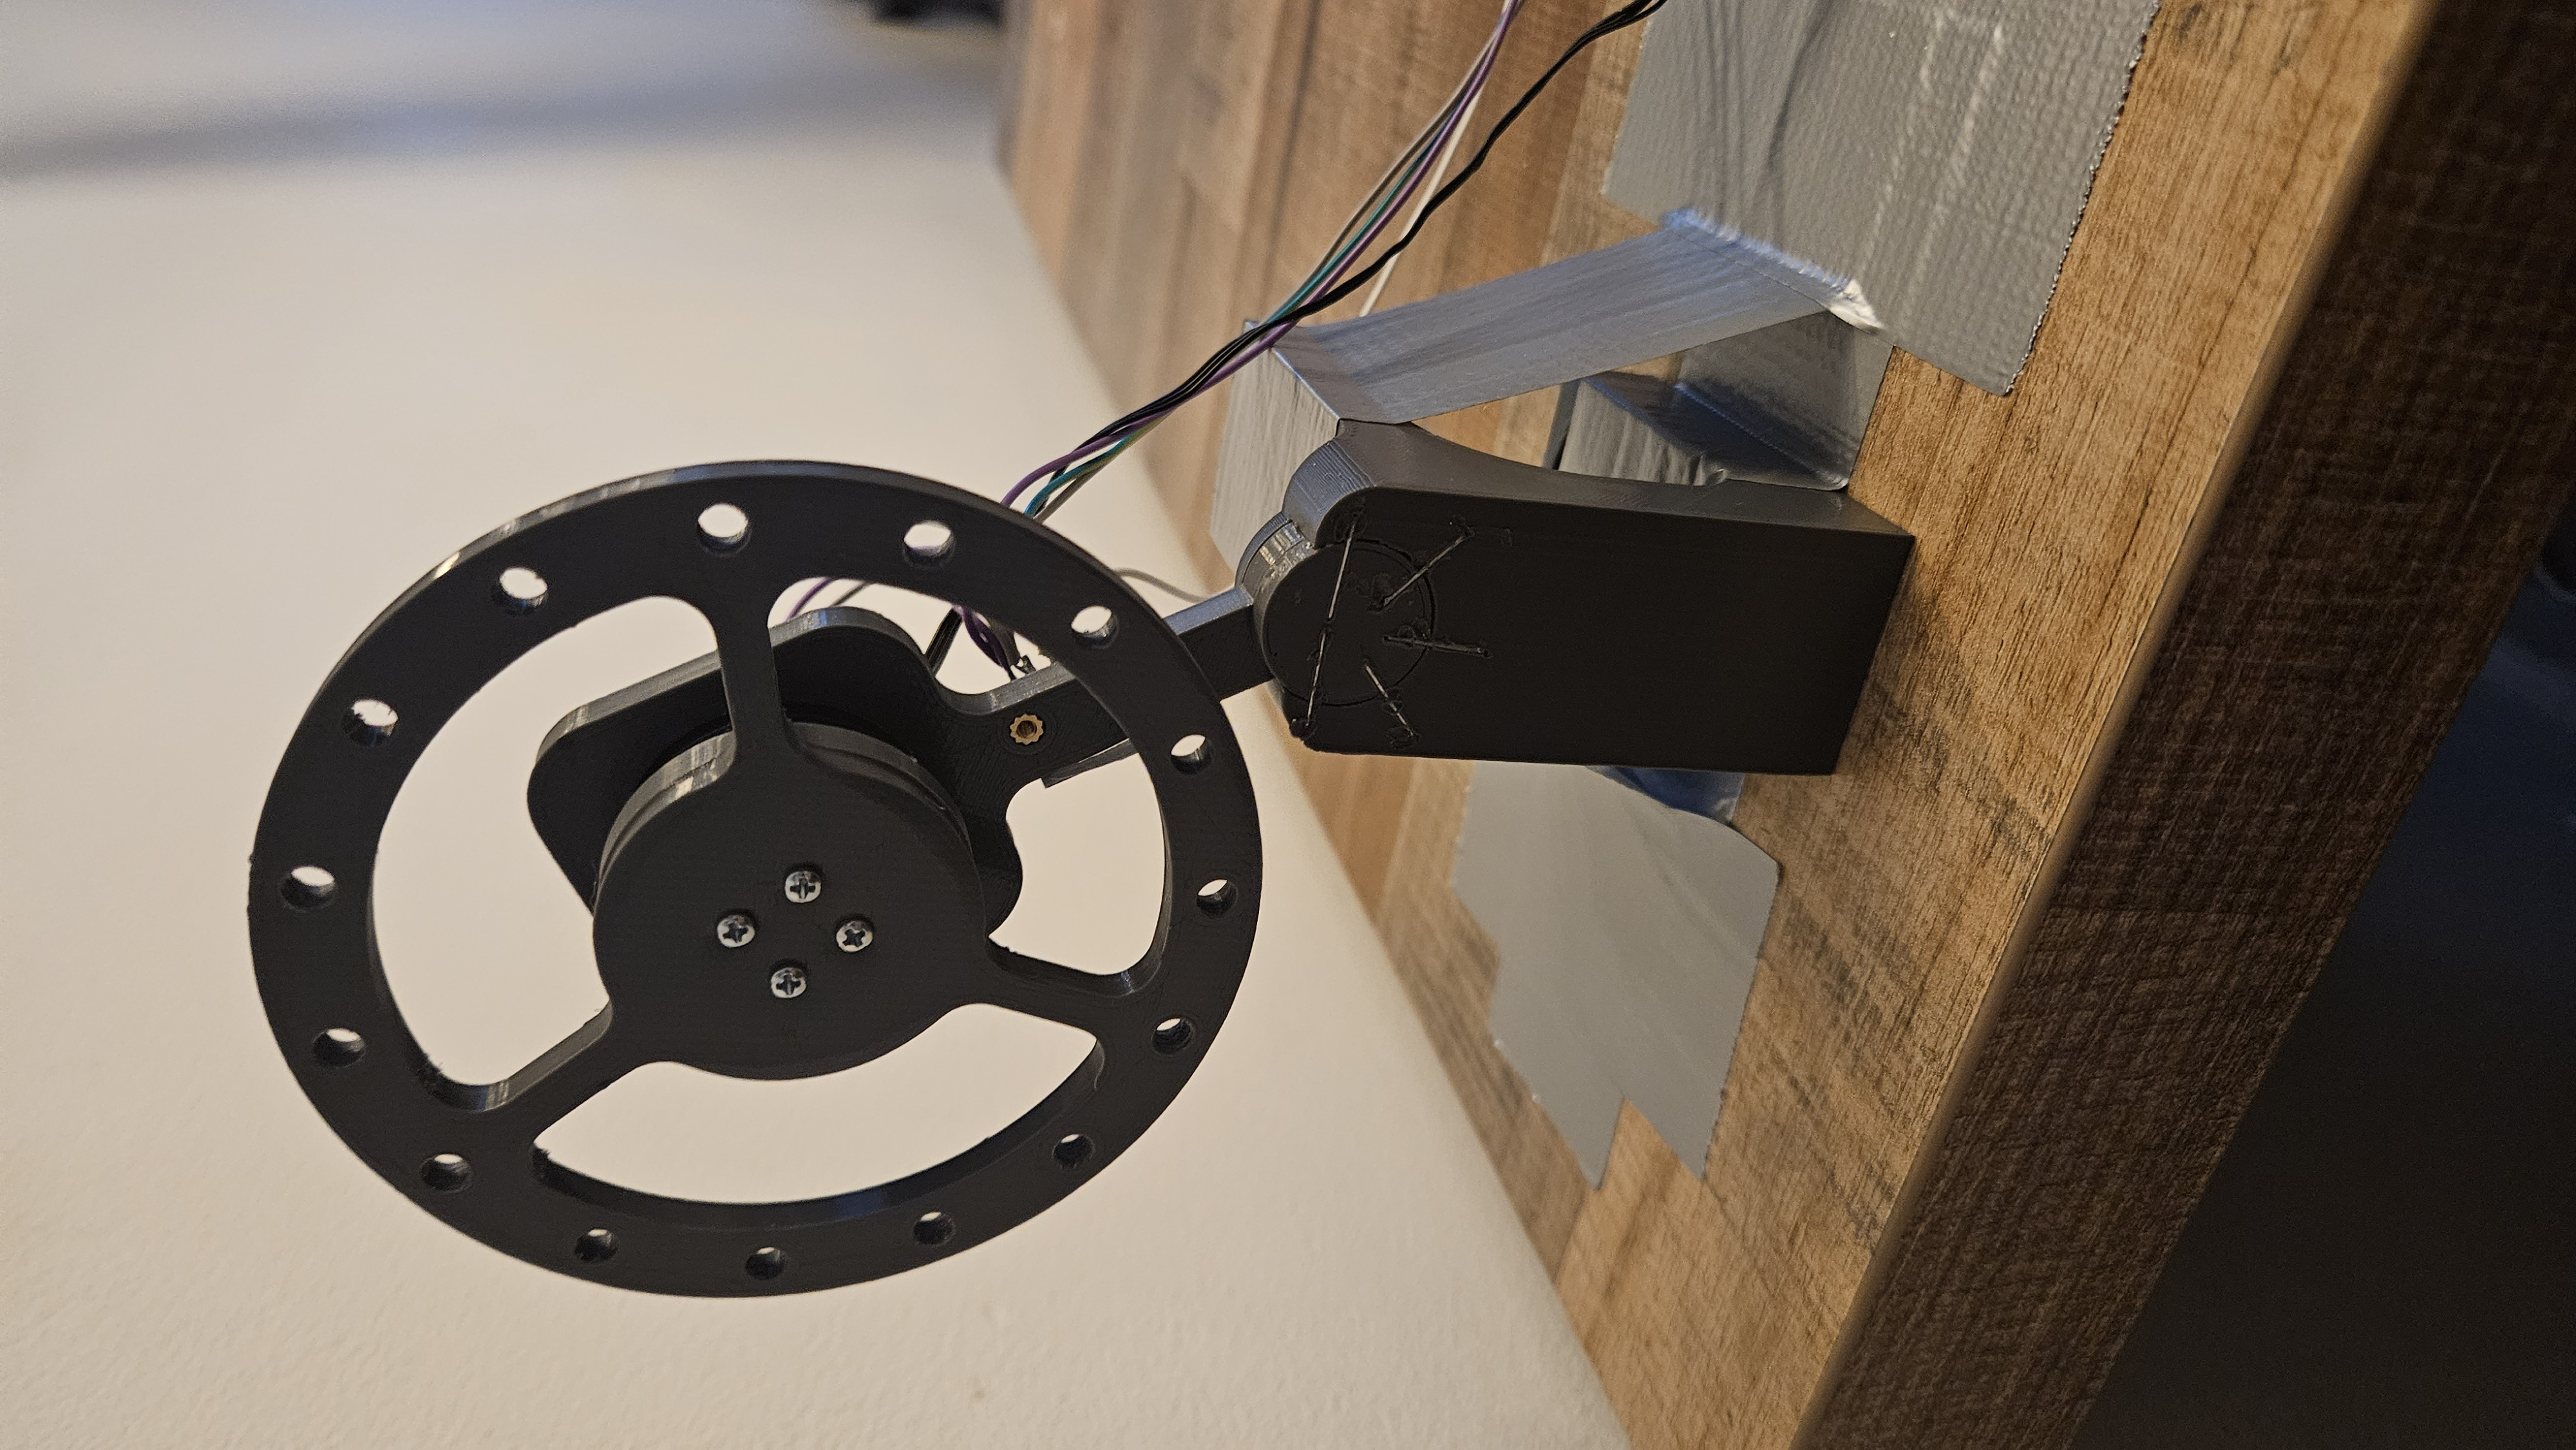
\includegraphics[scale=0.040, angle =-90 ]{20240114_155939}
\caption{Phisical setup.}
\label{fig:Phisical setup}
\end{figure}

Firstly, the gyro sensor that measures the angle of the pendulum. In the graph in figure \ref{fig:measurements gyro sensor}, you can see what the sensor measures. The deviation from the actual angle is too significant for this level of precision (up to a maximum of 2.75 degrees). However, an actual reading of the angle is crucial. If the actual angle of the pendulum is 0 degrees and the sensor reads 2 degrees, it will self-tilt. In a model like this, precision is crucial, where a deviation of 2 degrees can be fatal and may prevent it from maintaining balance.

\begin{figure}[H]
\centering
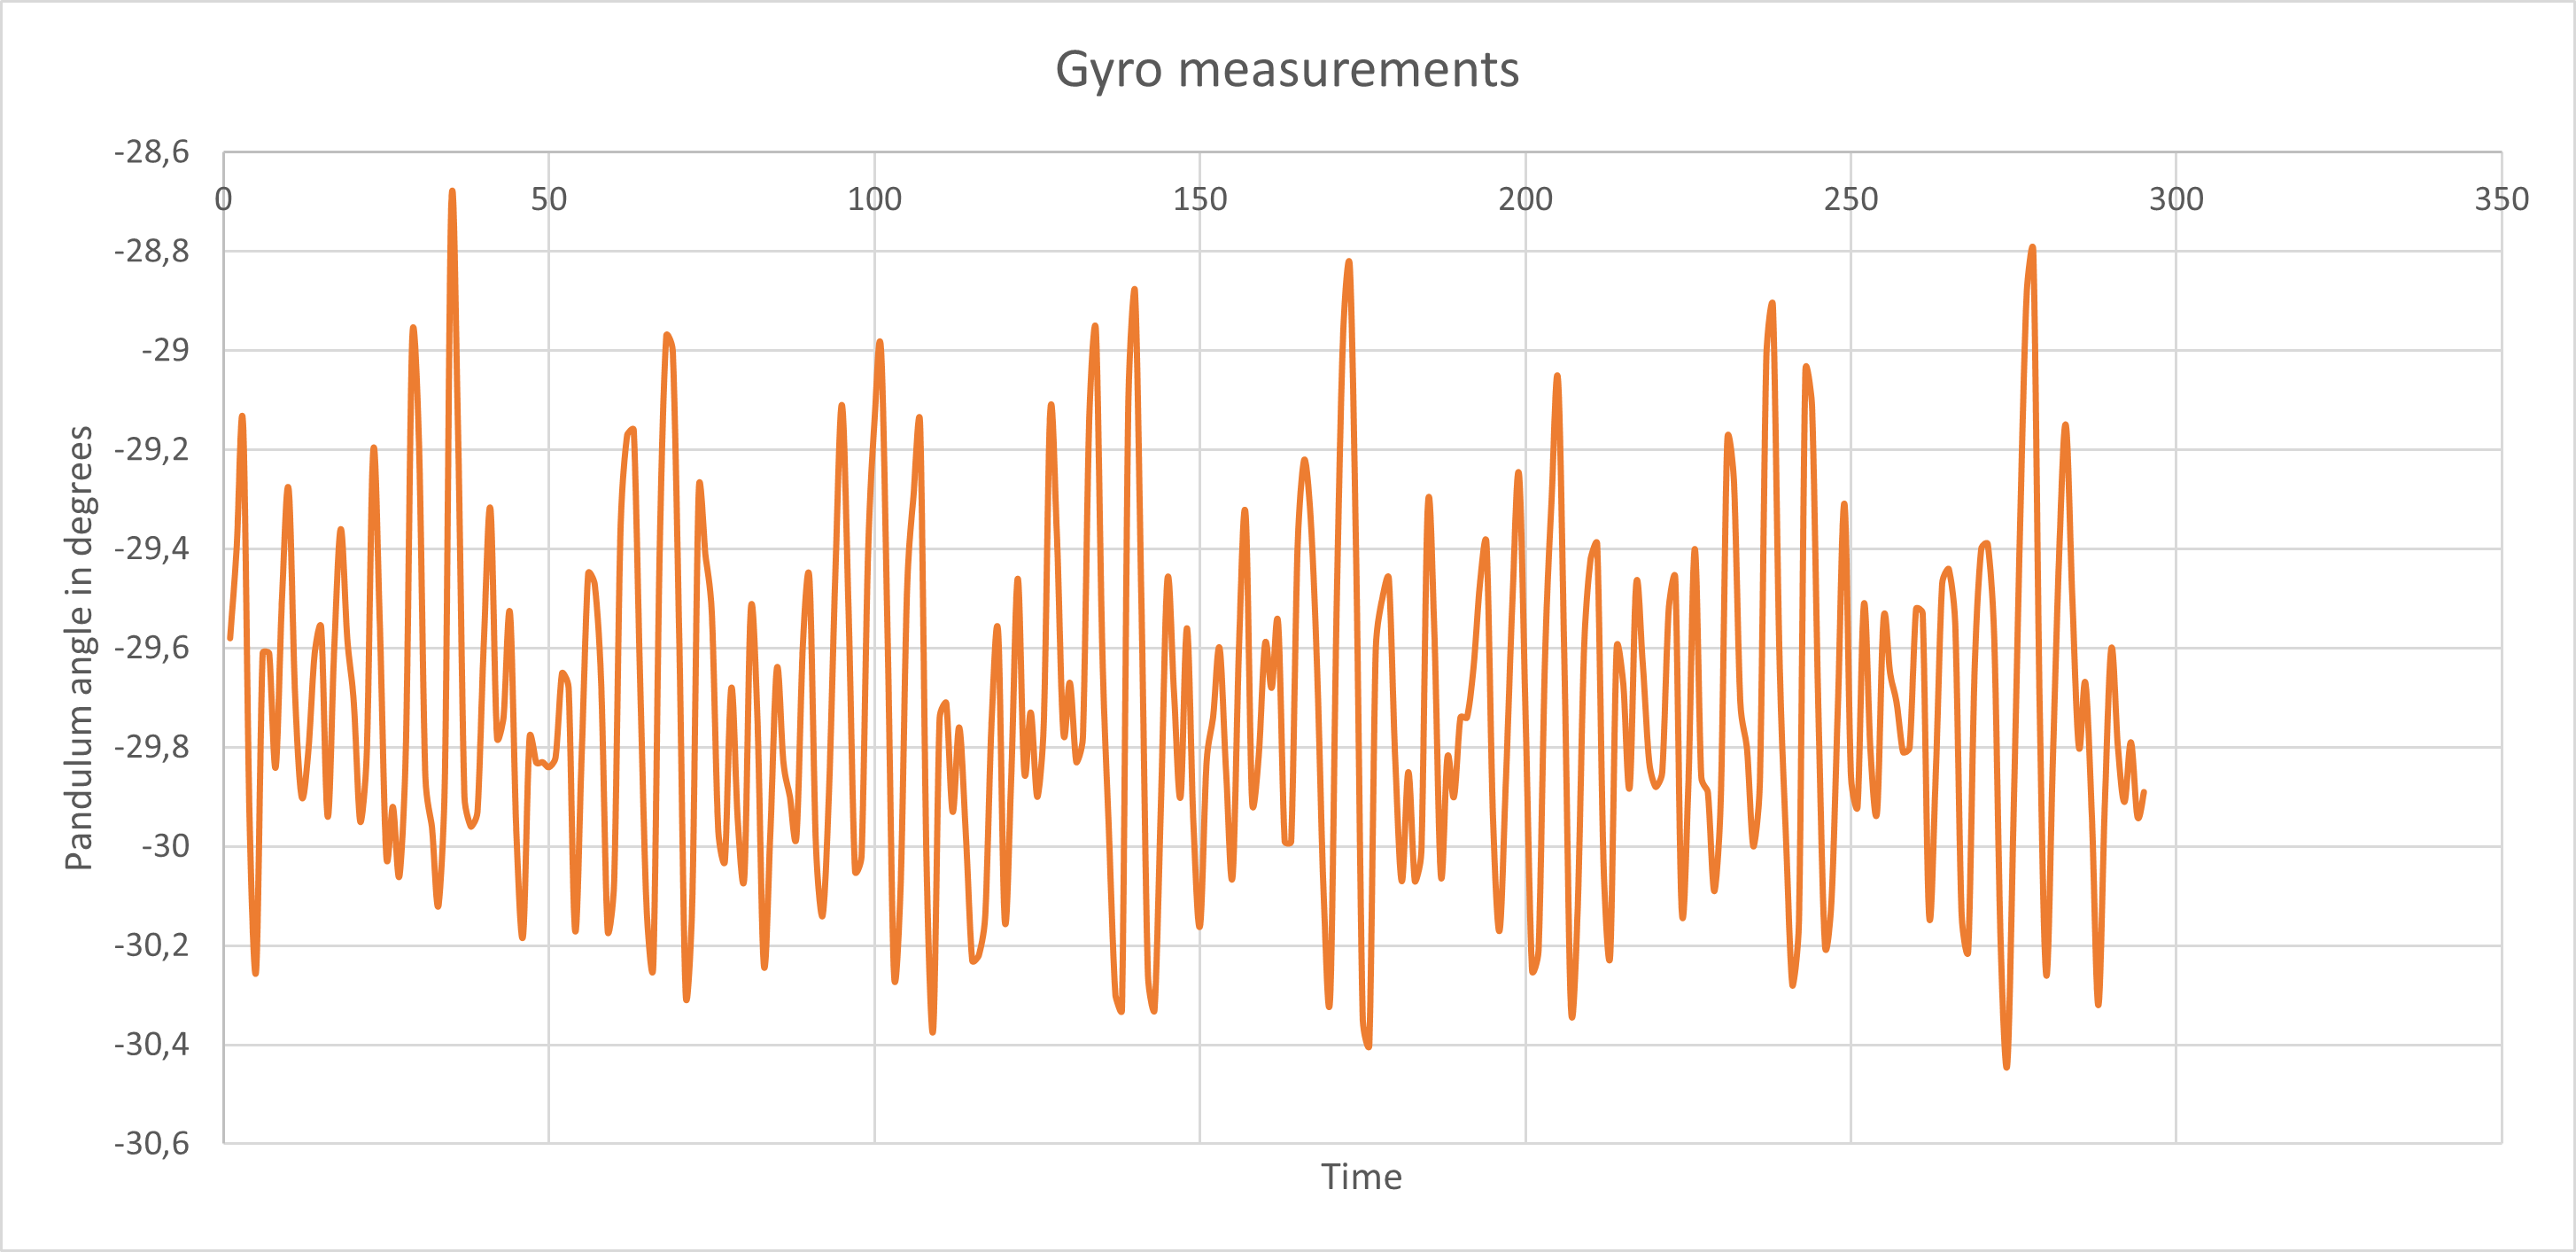
\includegraphics[scale=0.37]{Gyro meting}
\caption{measurements gyro sensor with no movement.}
\label{fig:measurements gyro sensor}
\end{figure}

What I didn't considered at the beginning of this project, in all my enthusiasm, is that the relatively small model results in a very small margin of error. This makes PID tuning extremely challenging. While in the simulation, you could see the pendulum beautifully oscillating towards its setpoint, achieving the same precision in reality, is proving to be quite difficult. This is partly due to the instability of the 3D-printed model and the sensor.

\begin{figure}[H]
\centering
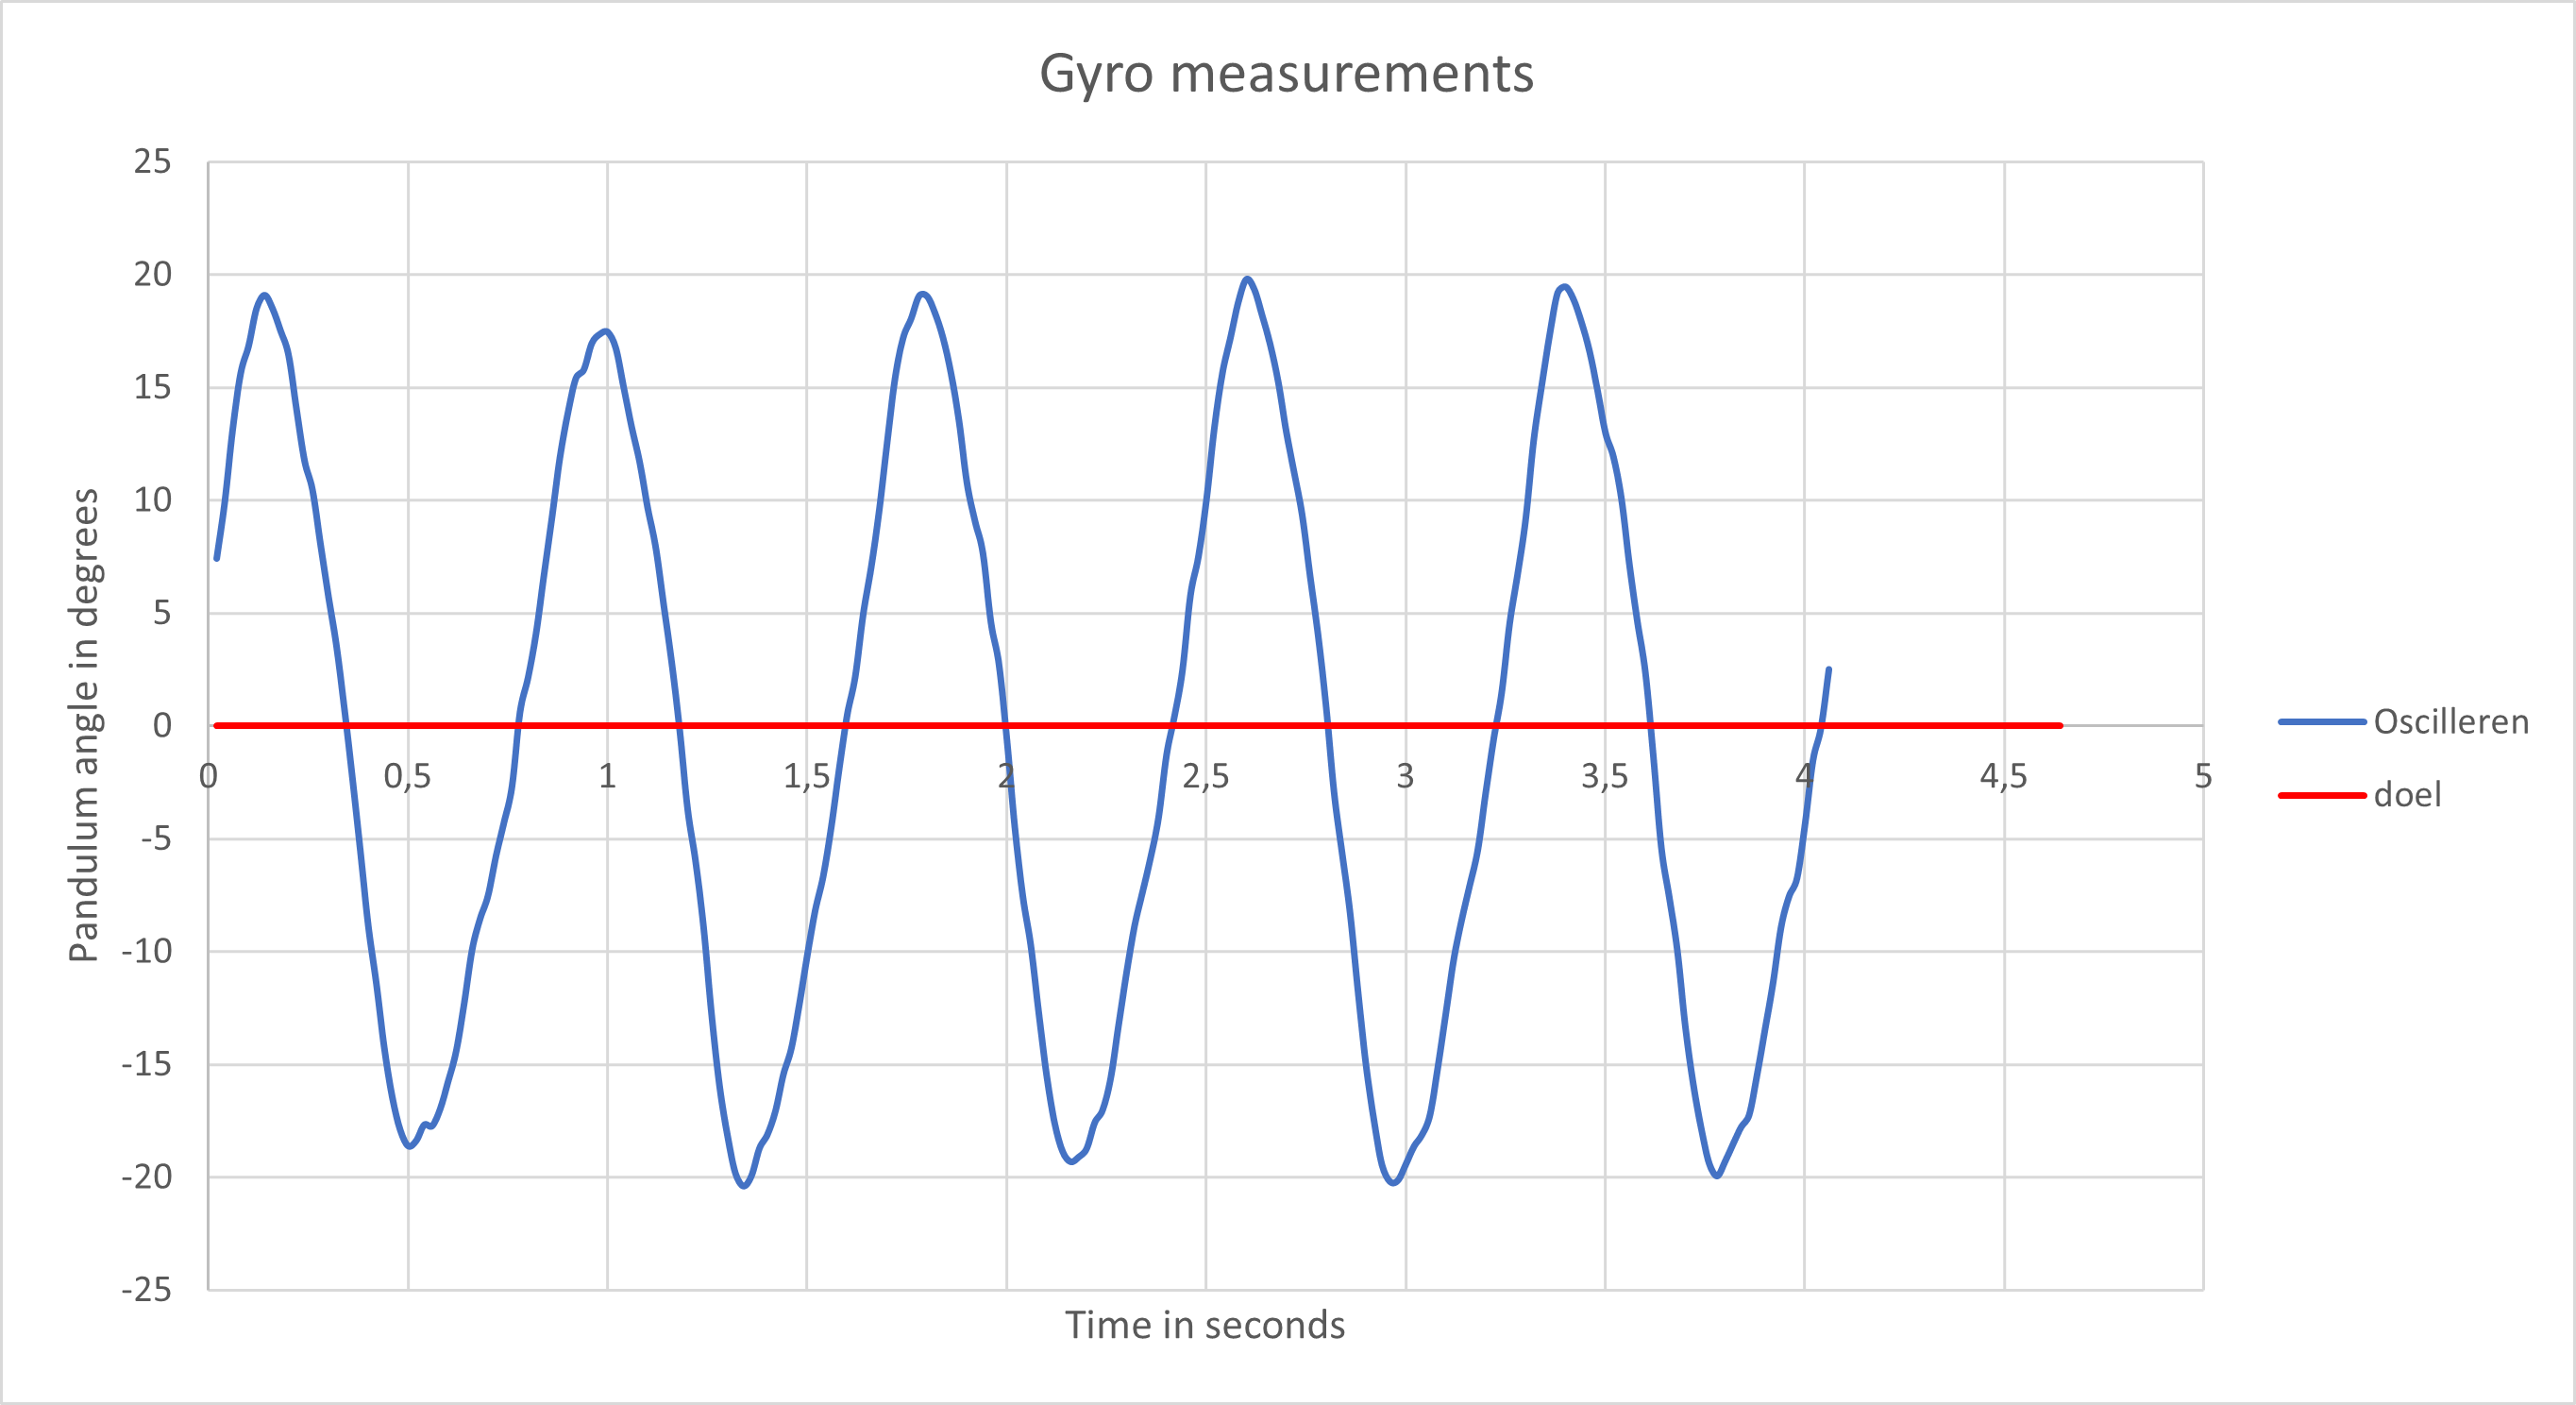
\includegraphics[scale=0.37]{Model Oscilating}
\caption{Phisical setup oscilating around its setpoint(0).}
\label{fig:Model oscilating to its setpoint(0)}
\end{figure}

\begin{figure}[H]
\centering
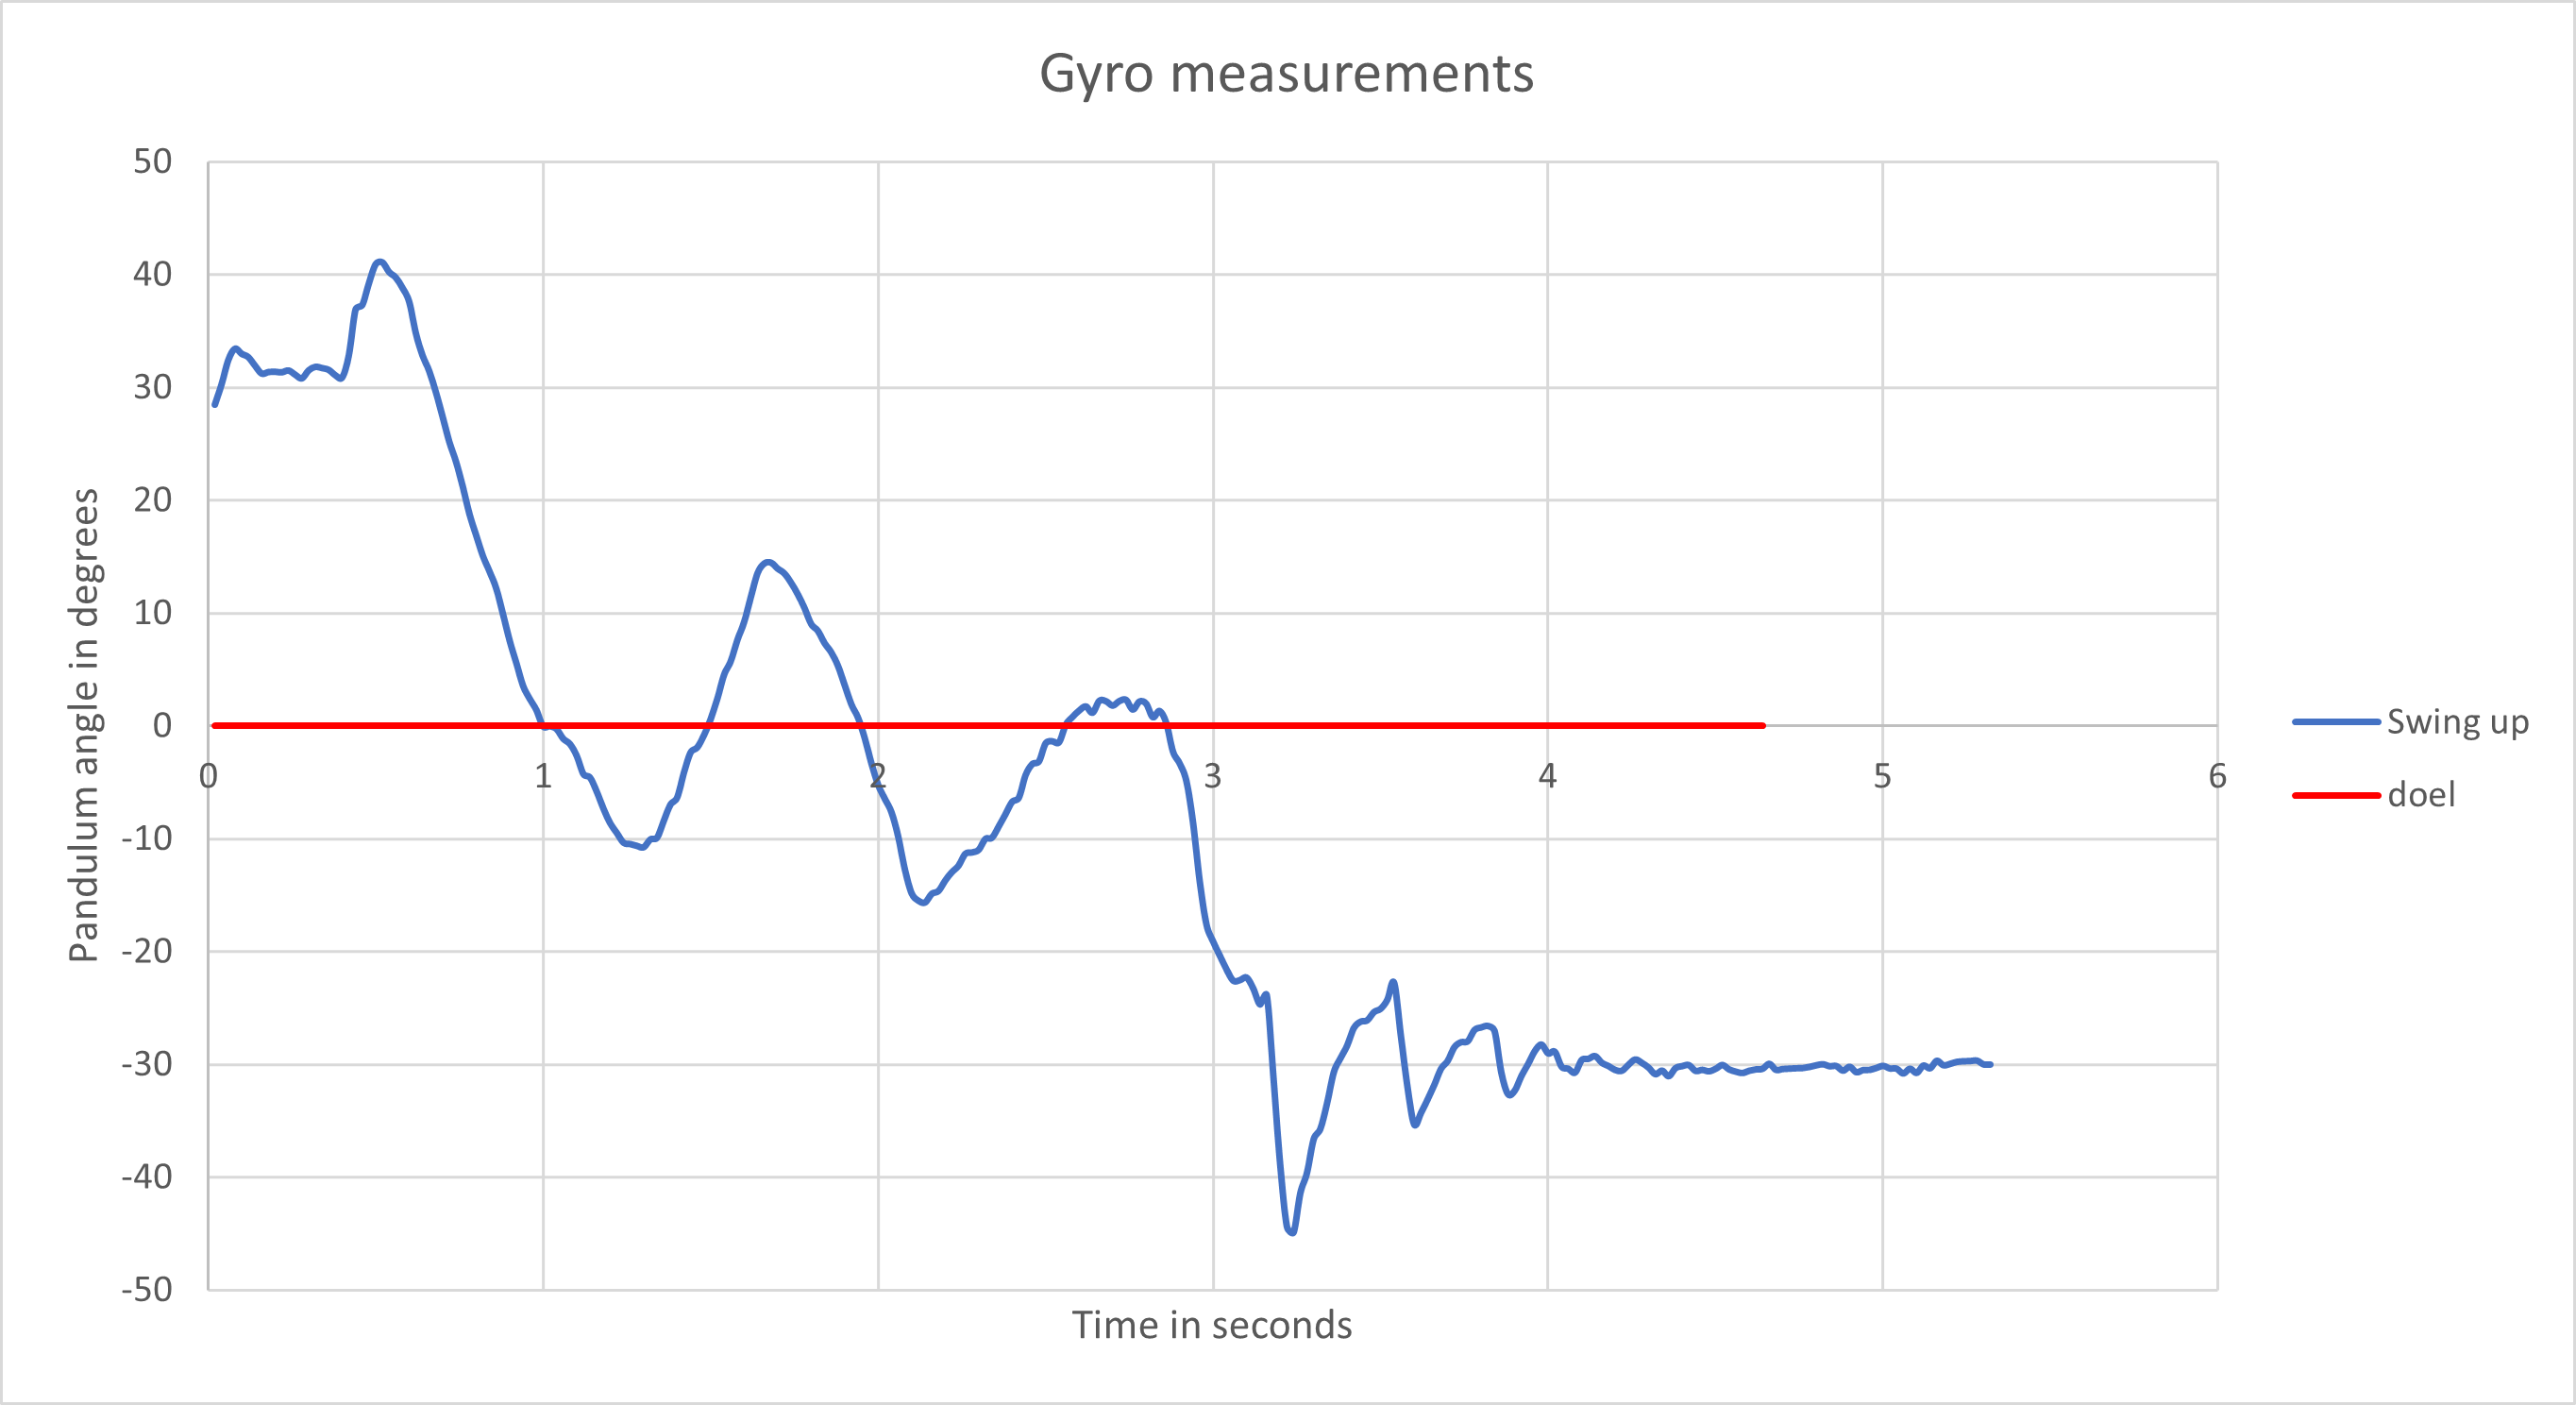
\includegraphics[scale=0.37]{Swing Up}
\caption{Phisical setup treis to make a swing up.}
\label{fig:swing up}
\end{figure}

I have conducted several measurements of the physical setup. In Figure \ref{fig:Model oscilating to its setpoint(0)}, you can observe how the physical setup oscillates around its setpoint. It struggles to approach the setpoint slowly, likely due to delayed measurements. Furthermore, in Figure \ref{fig:swing up}, you can see the swing-up phase. Once the pendulum is in its initial position, it attempts to swing itself upward by rapidly rotating the reaction wheel in one direction and then the other. This action generates a significant force to lift itself. However, as indicated in the graph, it fails to maintain balance on the setpoint. Consequently, the pendulum tilts over to the other side.

\begin{figure}[H]
\centering
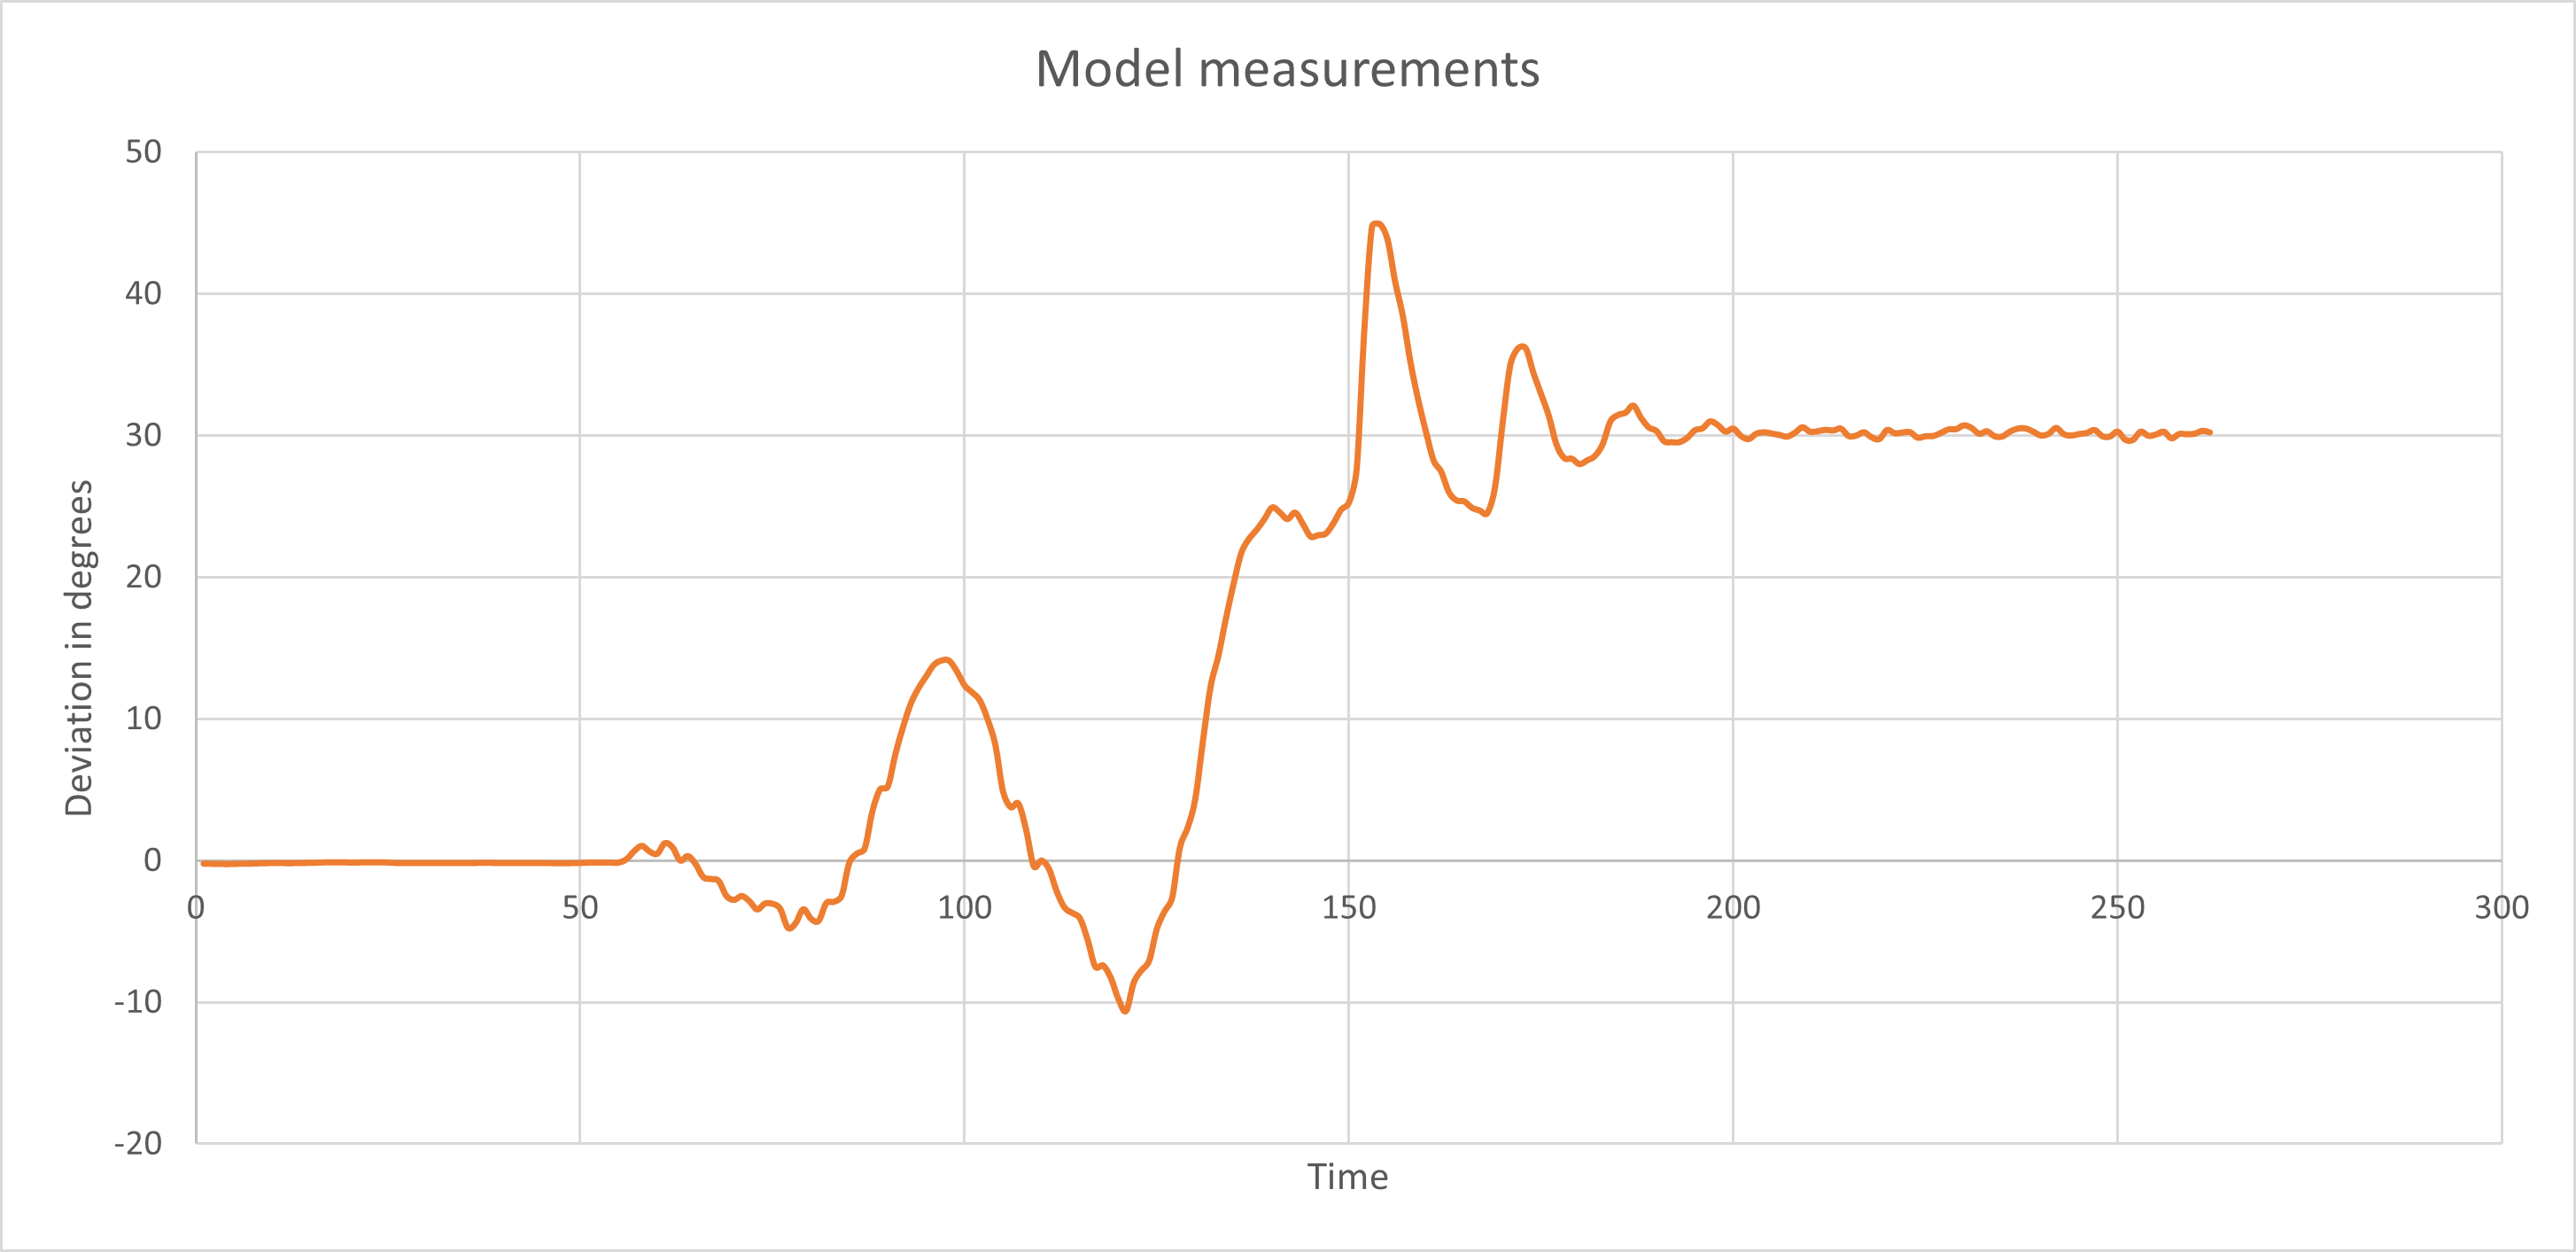
\includegraphics[scale=0.37]{Model stepresponse}
\caption{stepresponse of the phisical setup.}
\label{fig:stepresponse of the model}
\end{figure}

% \cite{deltap}


In the step response in figure \ref{fig:stepresponse of the model}, you can see how the pendulum initially reaches its setpoint, then experiences an external force, and struggles to balance back to its setpoint. This is likely due to insufficient precision, and the small margin of error prevents the system from responding quickly enough with accurate measurements. However, what is also noticeable, is that the sensor records very strange values at the end of the falling motion. This is visible in figure \ref{fig:stepresponse of the model} and \ref{fig:swing up} The pendulum can only fall to an angle of 30 degrees due to a mechanical blockage. In the graph, you can see the sensor registering an angle of almost 45 degrees during the fall, which is impossible. If the sensor frequently produces such incorrect measurements during balancing, I consider it impossible to achieve balance reliably with this sensor.

\vspace{.5cm}

If we trust the simulation, it should certainly be possible to balance a pendulum with a reaction wheel. We have also seen this in other practical examples on the internet. However, with the challenge of creating a relatively small model on a tight budget and using sensors that are not precise enough, this experiment has shown that achieving this goal is practically not feasible in the way I attempted it.

\subsection{Difference between the simulation and the physical setup}

It's interesting to observe the difference between the simulation and reality. While the model in the simulation works perfectly, the physical setup struggles to remain stable. When comparing graphs \ref{fig:Stepresponse PID controlled simulation Michel} and \ref{fig:Model oscilating to its setpoint(0)}, you can see that the simulation almost comes to a standstill at its setpoint, whereas the physical setup continues to oscillate around it. Clearly, there is a discrepancy, but upon closer inspection, you can notice some similarity in behavior. Unfortunately, the simulation cannot be fully compared to reality due to the following reasons. The simulation does not account for air resistance, and there is no consideration for friction in the pivot point of the pendulum. Additionally, the simulation does not incorporate the motor's properties.

\vspace{.5cm}

In the physical setup, there are several factors that hinder it from matching the simulation perfectly. The sensor provides inaccurate values, the small model allows little room for errors, and cable placement also affects the pendulum as they may "pull" on it if not properly arranged.

\vspace{.5cm}

Addressing all these factors would likely lead to a closer resemblance between the simulation and the physical setup.

\section{Conclusions and recommendations}
Conclusions:
\begin{itemize}
\item An experimental setup was created to attempt balancing a pendulum with a reaction wheel using PID control.
\item Different controller settings were tried and a optimal setting was found. 
\item A digital twin was made of the setup in python.  
\end{itemize}
Recommendations:
\begin{itemize}
\item Create a larger model so that there is more room for error.
\item Using a different sensor, such as the AS5600, for a more precise angle measurement. 
\item Constructing a sturdier model with less friction at the pivot point.
\end{itemize}


\section{Bibliography}
\begin{enumerate}
    \item \textbf{YouTube} How to build self balancing Cube \href{https://www.youtube.com/watch?v=AJQZFHJzwt4}{https://www.youtube.com}
    \item \textbf{YouTube} Self balancing bike  \href{https://www.youtube.com/watch?v=Je9Y2WaRB6g&t=7s}{https://www.youtube.com}
    \item \textbf{YouTube} Self balancing triangle (reaction wheel)  \href{https://www.youtube.com/watch?v=dTYiqNcXw68&t=154s}{https://www.youtube.com}
    \item \textbf{YouTube} A Lesson in Failure: Reaction Wheel PID Tuning \href{https://www.youtube.com/watch?v=kMCPTmi7f-4&list=PLMAbfx2u_zm4uqeRiwqP0UWDNL2hisYsA&index=6&t=721s}{https://www.youtube.com}
    \item \textbf{PDF} Kinematics Proposal.pdf  \href{https://github.com/B-Paweekorn/Reaction-wheel-inverted-pendulum/blob/main/Kinematics%20Proposal.pdf}{Reaction-wheel-inverted-pendulum/blob/main/Kinematics20Proposal.pdf}
    \item \textbf{GitHub} GitHub Remigijus  \href{https://github.com/remrc/}{https://github.com/remrc/}
\end{enumerate}
\end{multicols}
\newpage

%Bibliography
\bibliographystyle{IEEEtran}
\bibliography{bib}
\appendix


%Bijlages
\section{Code used for controlling the setup}
%New colors defined below
\definecolor{codegreen}{rgb}{0,0.6,0}
\definecolor{codegray}{rgb}{0.5,0.5,0.5}
\definecolor{codepurple}{rgb}{0.58,0,0.82}
\definecolor{backcolour}{rgb}{0.95,0.95,0.92}

%Code listing style named "mystyle"
\lstdefinestyle{mystyle}{
  backgroundcolor=\color{backcolour}, commentstyle=\color{codegreen},
  keywordstyle=\color{magenta},
  numberstyle=\tiny\color{codegray},
  stringstyle=\color{codepurple},
  basicstyle=\ttfamily\footnotesize,
  breakatwhitespace=false,         
  breaklines=true,                 
  captionpos=b,                    
  keepspaces=true,                 
  numbers=left,                    
  numbersep=5pt,                  
  showspaces=false,                
  showstringspaces=false,
  showtabs=false,                  
  tabsize=2
}
\lstset{style=mystyle}
\begin{lstlisting}[language=C, caption=Arduino Nano Code]
void MPUsetup();
void MPUread(float *GyroX, float *GyroY, float *GyroZ);
float PID_Controller(float angle, float accel);

#include <SimpleFOC.h>
#include <Adafruit_MPU6050.h>
#include <Adafruit_Sensor.h>
#include <Wire.h>

Adafruit_MPU6050 mpu;

#define PIE 3.14159265358979323846   // define pi
#define RAD_TO_DEG 57.295779513082320876798154814105 // 180/pi
#define MICROSECONDS_TO_SECONDS 1000000.0 // 1 million

// global variables
float angleX = 0, angleY = 0, angleZ = 0;
float GyroX, GyroY, GyroZ;
float correctie = 0.0;
unsigned long lastTime = 0;
float previous_angle = 0;

// magnetic sensor instance - SPI
// MagneticSensorSPI sensor = MagneticSensorSPI(AS5147_SPI, 10);
// magnetic sensor instance - I2C
MagneticSensorI2C sensor = MagneticSensorI2C(AS5600_I2C);
// magnetic sensor instance - analog output
// MagneticSensorAnalog sensor = MagneticSensorAnalog(A1, 14, 1020);

// BLDC motor & driver instance
BLDCMotor motor = BLDCMotor(7);
BLDCDriver3PWM driver = BLDCDriver3PWM(9, 10, 11);
// Stepper motor & driver instance
//StepperMotor motor = StepperMotor(50);
//StepperDriver4PWM driver = StepperDriver4PWM(9, 5, 10, 6,  8);

// voltage set point variable
// // instantiate the commander
// Commander command = Commander(Serial);
// void doTarget(char* cmd) { command.scalar(&target_voltage, cmd); }

void setup() {

  // initialise magnetic sensor hardware
  sensor.init();
  // link the motor to the sensor
  motor.linkSensor(&sensor);

  // power supply voltage
  driver.voltage_power_supply = 12;
  driver.init();
  motor.linkDriver(&driver);

  // aligning voltage 
  motor.voltage_sensor_align = 5;
  // choose FOC modulation (optional)
  motor.foc_modulation = FOCModulationType::SpaceVectorPWM;
  // set motion control loop to be used
  motor.controller = MotionControlType::torque;

  // use monitoring with serial 
  Serial.begin(115200);
  // // comment out if not needed
  // motor.useMonitoring(Serial);

  // initialize motor
  motor.init();
  // align sensor and start FOC
  motor.initFOC();

    MPUsetup();
  for (int i = 0; i < 10; i++) {
    MPUread(&GyroX, &GyroY, &GyroZ);
  }

  if (GyroX < -90){
    correctie = -29.5-GyroX;
  }
  else{
    correctie = 29.5-GyroX;
  }

  // // add target command T
  // command.add('T', doTarget, "target voltage");

  Serial.println(F("Motor ready."));
  Serial.println(F("Set the target voltage using serial terminal:"));
  _delay(1000);
}

void loop() {
  float target_voltage = 0;
  float acceleratie_p = 0;
  MPUread(&GyroX, &GyroY, &GyroZ);
  GyroX+=correctie;
  acceleratie_p = GyroX-previous_angle;

  target_voltage = PID_Controller(GyroX, acceleratie_p);
  motor.loopFOC();
  motor.move(target_voltage);

  // Serial.print("vorige hoek: "); Serial.print(previous_angle);Serial.print(" hoek: "); Serial.print(GyroX);Serial.print(" acceleratie: "); Serial.println(acceleratie_p);
  Serial.println(GyroX);
  previous_angle = GyroX;
}

float PID_Controller(float angle, float accel) {
  // PID gains for angle
  float Kp_angle = 1.4; // 1.4
  float Ki_angle = 0.0;  // Add I term
  float Kd_angle = 3.6; // 3.6

  // PID gains for acceleration
  float Kp_accel = 0.0;
  float Ki_accel = 0.0;
  float Kd_accel = 0.0;
  
  int error_angle, integral_angle, derivative_angle;
  int error_accel, integral_accel, derivative_accel;
  
  float voltage;

  // Static variables to store previous errors
  static int prev_error_angle = 0;
  static int prev_error_accel = 0;

  // Calculate error for angle
  error_angle = 0 - angle;
  integral_angle += error_angle;
  derivative_angle = error_angle - prev_error_angle;

  // Calculate error for acceleration
  error_accel = 0 - accel;
  integral_accel += error_accel;
  derivative_accel = error_accel - prev_error_accel;

  // Calculate control inputs using PID
  float control_angle = Kp_angle * error_angle + Ki_angle * integral_angle + Kd_angle * derivative_angle;
  float control_accel = Kp_accel * error_accel + Ki_accel * integral_accel + Kd_accel * derivative_accel;

  // Combine the control inputs
  voltage = control_angle + control_accel;

  // Update previous errors for the next iteration
  prev_error_angle = error_angle;
  prev_error_accel = error_accel;

  return voltage;
}



void MPUsetup(){
    // this function is called in main setup to initialize the MPU6050
    if (!mpu.begin())
    {
        Serial.println(F("Failed to find MPU6050 chip"));
        while (1)
        {
            delay(10);
        }
    }
    Serial.println(F("MPU6050 Found!"));

    // test code
    mpu.setAccelerometerRange(MPU6050_RANGE_4_G);
    Serial.print("Accelerometer range set to: ");
    switch (mpu.getAccelerometerRange())
    {
    case MPU6050_RANGE_2_G:
        Serial.println("+-2G");
        break;
    case MPU6050_RANGE_4_G:
        Serial.println("+-4G");
        break;
    case MPU6050_RANGE_8_G:
        Serial.println("+-8G");
        break;
    case MPU6050_RANGE_16_G:
        Serial.println("+-16G");
        break;
    }
    mpu.setGyroRange(MPU6050_RANGE_250_DEG);
    Serial.print("Gyro range set to: ");
    switch (mpu.getGyroRange())
    {
    case MPU6050_RANGE_250_DEG:
        Serial.println("+- 250 deg/s");
        break;
    case MPU6050_RANGE_500_DEG:
        Serial.println("+- 500 deg/s");
        break;
    case MPU6050_RANGE_1000_DEG:
        Serial.println("+- 1000 deg/s");
        break;
    case MPU6050_RANGE_2000_DEG:
        Serial.println("+- 2000 deg/s");
        break;
    }

    mpu.setFilterBandwidth(MPU6050_BAND_5_HZ);
    Serial.print("Filter bandwidth set to: ");
    switch (mpu.getFilterBandwidth())
    {
    case MPU6050_BAND_260_HZ:
        Serial.println("260 Hz");
        break;
    case MPU6050_BAND_184_HZ:
        Serial.println("184 Hz");
        break;
    case MPU6050_BAND_94_HZ:
        Serial.println("94 Hz");
        break;
    case MPU6050_BAND_44_HZ:
        Serial.println("44 Hz");
        break;
    case MPU6050_BAND_21_HZ:
        Serial.println("21 Hz");
        break;
    case MPU6050_BAND_10_HZ:
        Serial.println("10 Hz");
        break;
    case MPU6050_BAND_5_HZ:
        Serial.println("5 Hz");
        break;
    }
}

void MPUread(float *GyroX, float *GyroY, float *GyroZ){
    // if called by main this function will read IMU data from the MPU6050 and return it
    sensors_event_t a, g, temp;
    mpu.getEvent(&a, &g, &temp);

    unsigned long currentTime = micros();
    float dt = (currentTime - lastTime) / MICROSECONDS_TO_SECONDS; // convert to seconds
    lastTime = currentTime;

    // calculate angle based on gyro data
    float gyroAngleX = angleX + g.gyro.x * dt;
    // float gyroAngleY = angleY + g.gyro.y * dt;
    // float gyroAngleZ = angleZ + g.gyro.z * dt;

    // calculate angle based on accelerometer data
    float accelAngleX = atan2(a.acceleration.y, a.acceleration.z);
    // float accelAngleY = atan2(a.acceleration.x, a.acceleration.z);

    // complementary filter: combine the gyro and accelerometer angles
    float alpha = 0.5; // weight factor
    angleX = alpha * gyroAngleX + (1.0 - alpha) * accelAngleX;
    // angleY = alpha * gyroAngleY + (1.0 - alpha) * accelAngleY;
    // angleZ = gyroAngleZ; // gyro only on Z axis

    angleX += g.gyro.x * dt;
    // angleY += g.gyro.y * dt;
    // angleZ += g.gyro.z * dt;

    // convert angles from radians to degrees
    *GyroX = -((angleX * RAD_TO_DEG));
    // *GyroY = angleY * RAD_TO_DEG;
    // *GyroZ = angleZ * RAD_TO_DEG;
    *GyroY = 0;
    *GyroZ = 0;
    // Serial.print(" GyroX: ");
    // Serial.print(*GyroX);
    // Serial.print(" GyroY: ");
    // Serial.print(*GyroY);
    // Serial.println("Degrees");
}
\end{lstlisting}
\newpage
\section{Code use for the simulation setup}
%New colors defined below
\definecolor{codegreen}{rgb}{0,0.6,0}
\definecolor{codegray}{rgb}{0.5,0.5,0.5}
\definecolor{codepurple}{rgb}{0.58,0,0.82}
\definecolor{backcolour}{rgb}{0.95,0.95,0.92}

%Code listing style named "mystyle"
\lstdefinestyle{mystyle}{
  backgroundcolor=\color{backcolour}, commentstyle=\color{codegreen},
  keywordstyle=\color{magenta},
  numberstyle=\tiny\color{codegray},
  stringstyle=\color{codepurple},
  basicstyle=\ttfamily\footnotesize,
  breakatwhitespace=false,         
  breaklines=true,                 
  captionpos=b,                    
  keepspaces=true,                 
  numbers=left,                    
  numbersep=5pt,                  
  showspaces=false,                
  showstringspaces=false,
  showtabs=false,                  
  tabsize=2
}
\lstset{style=mystyle}
\begin{lstlisting}[language=Python, caption=Python simulation]

import pygame
import math
import numpy as np

REFRESHRATE = 120 #[Hz]
pygame.init()
win_width, win_height = 1200, 800
win = pygame.display.set_mode((win_width,win_height))
pygame.display.set_caption("Reaction Wheel")
clock = pygame.time.Clock()  # For controlling the frame rate
# Font initialization
font = pygame.font.Font(None, 20)  # You can specify a font file or use None for default font and size
run = True

# global physics variables
MASSA_REACTIONWHEEL = 0.1 #[kg]
RADIUS_REACTIONWHEEL = 0.005 #[m]
LENGTE_PENDULUM = 0.1 #[m]
MASSA_PENDULUM = 0.2 #[kg]
GRAVITATIE_CONSTANTE = 9.81 #[m/s^2]

Torque_Gravity = 0 #[Nm]

ALPHA_RACTIONWHEEL = 0 #[rad/s^2] hoekverscnelling
OMEGA_REACTIONWHEEL = 0 #[rad/s] hoeksnelheid
THETA_REACTIONWHEEL = 0 #[rad] hoek

ALPHA_PENDULUM = 0 #[rad/s^2] hoekverscnelling
OMEGA_PENDULUM = 0 #[rad/s] hoeksnelheid
THETA_PENDULUM = 0 #[rad] hoek

THETA_PENDULUM = np.pi*-0.5
hoek_pendulum = 0

# Initialize global variables
integral = 0
prev_error = 0



def physics():
    global ALPHA_PENDULUM, OMEGA_PENDULUM, THETA_PENDULUM, OMEGA_REACTIONWHEEL, THETA_REACTIONWHEEL, Torque_Gravity, hoek_pendulum
    
    # Inertia calculations
    Inertia_ReactionWheel = (MASSA_REACTIONWHEEL*(RADIUS_REACTIONWHEEL**2))/2
    Inertia_Pendulum = (1/3)*MASSA_PENDULUM*(LENGTE_PENDULUM**2)

    # Torque CALCULATIONS
    Torque_ReactionWheel = ALPHA_RACTIONWHEEL * Inertia_ReactionWheel
    Torque_Gravity = (MASSA_REACTIONWHEEL+MASSA_PENDULUM) * GRAVITATIE_CONSTANTE * np.cos(THETA_PENDULUM)

    # Main CalCul
    #ALPHA_PENDULUM = Torque_ReactionWheel+Torque_Gravity/Inertia_Pendulum+MASSA_REACTIONWHEEL*(LENGTE_PENDULUM**2)

    total_torque = Torque_ReactionWheel + Torque_Gravity
    total_inertia = Inertia_Pendulum + MASSA_REACTIONWHEEL * (LENGTE_PENDULUM**2)

    ALPHA_PENDULUM = total_torque / total_inertia

    #intergrations
    OMEGA_PENDULUM += ALPHA_PENDULUM * 1/REFRESHRATE
    THETA_PENDULUM += OMEGA_PENDULUM * 1/REFRESHRATE
    hoek_pendulum = (THETA_PENDULUM*180/np.pi)+90

    OMEGA_REACTIONWHEEL += ALPHA_RACTIONWHEEL*1/REFRESHRATE
    THETA_REACTIONWHEEL += OMEGA_REACTIONWHEEL*1/REFRESHRATE

    if hoek_pendulum > 360:
        THETA_PENDULUM = np.pi*-0.5



def pid_controller(hoek):
    global integral, prev_error  # Assuming these are used elsewhere and need to be shared

    # PID constants
    Kp = 5.43
    Ki = 0.0
    Kd = 12.0

    # Initialize variables
    error = 0 - hoek  # Calculate the error
    integral += error  # Calculate the integral

    # Calculate the derivative term
    derivative = error - prev_error

    # PID calculation
    draai = Kp * error + Ki * integral + Kd * derivative  # Calculate the control output

    # Update the previous error for the next iteration
    prev_error = error

    return draai


while run:
    pygame.time.delay(20)

    for event in pygame.event.get():
        if event.type == pygame.QUIT:
            run = False

    keys = pygame.key.get_pressed()
    if keys[pygame.K_LEFT]:
        ALPHA_RACTIONWHEEL -= 1
    elif keys[pygame.K_RIGHT]:
        ALPHA_RACTIONWHEEL += 1
    elif keys[pygame.K_SPACE]:
        # Reset all relevant variables to their initial values
        ALPHA_RACTIONWHEEL = 0
        OMEGA_REACTIONWHEEL = 0
        THETA_REACTIONWHEEL = 0
        ALPHA_PENDULUM = 0
        OMEGA_PENDULUM = 0
        THETA_PENDULUM = np.pi*-.5  # Set to initial angle
        Torque_Gravity = 0
        Torque_ReactionWheel = 0
        Inertia_ReactionWheel = 0
        Inertia_Pendulum = 0

    ALPHA_RACTIONWHEEL = pid_controller(hoek_pendulum)

    physics()


    # Fixed point coordinates (center of rotation)
    center_x, center_y = (win_width/2), (win_height/2)
    # Stick length
    stick_length = 200
    # Calculate the endpoint of the stick based on the angle
    end_x = center_x + stick_length * np.cos(THETA_PENDULUM)
    end_y = center_y + stick_length * np.sin(THETA_PENDULUM)
    
    text_to_display1 = f"ALPHA_PENDULUM: {ALPHA_PENDULUM}"
    text_1= font.render(text_to_display1, True, (255, 0, 0))
    text_to_display2 = f"OMEGA_PENDULUM: {OMEGA_PENDULUM}"
    text_2= font.render(text_to_display2, True, (255, 0, 0))
    text_to_display3 = f"hoek_pendulum: {hoek_pendulum}"
    text_3= font.render(text_to_display3, True, (255, 0, 0))
    text_to_display4 = f"ALPHA_REACTIONWHEEL: {ALPHA_RACTIONWHEEL}"
    text_4= font.render(text_to_display4, True, (255, 0, 0))
    text_to_display5 = f"OMEGA_REACTIONWHEEL: {OMEGA_REACTIONWHEEL}"
    text_5= font.render(text_to_display5, True, (255, 0, 0))
    text_to_display6 = f"THETA_REACTIONWHEEL: {THETA_REACTIONWHEEL}"
    text_6= font.render(text_to_display6, True, (255, 0, 0))
    text_to_display7 = f"Torque_Gravity: {Torque_Gravity}"
    text_7= font.render(text_to_display7, True, (255, 0, 0))

    win.fill((0, 0, 0))

    # Blit the text onto the window surface at (x, y) position
    win.blit(text_1, (50, 50))  # Adjust position as needed
    win.blit(text_2, (50, 60))  # Adjust position as needed
    win.blit(text_3, (50, 70))  # Adjust position as needed
    win.blit(text_4, (50, 80))  # Adjust position as needed
    win.blit(text_5, (50, 90))  # Adjust position as needed
    win.blit(text_6, (50, 100))  # Adjust position as needed
    win.blit(text_7, (50, 110))  # Adjust position as needed

    pygame.draw.line(win, (0, 255, 0), (0, center_y+25), (win_width, center_y+25), 50)
    pygame.draw.line(win, (255, 255, 255), (center_x, center_y), (end_x, end_y), 5)
    pygame.display.update()
    clock.tick(REFRESHRATE)  # Limit frame rate 
    
pygame.quit()
\end{lstlisting}
\newpage
\end{document}